\chapter{Time Series Methods for Air Quality}

With the proliferation of low-cost sensors for a wide range of IoT and wearable biometric applications, a systematic approach to both quality control and performing comprehensive time series analysis has significant value. It is highly desirable to be able to answer some basic questions using \textit{just} the time series alone. For example: What is the likely sensor uncertainty given a time series of observations? How frequently should observations be made to adequately resolve typical temporal variability? How representative is a single observation of what one expects to see over a temporal (and spatial) window? Can we construct predictive models for the time series of a single sensor given a sufficient volume of sample data? I this chapter we seek to address these questions with direct application to the data collected by our low cost air quality sensor network. First, we will demonstrate how the \textit{temporal variogram} provides a way to assess the intrinsic sensor uncertainty from a time series. Next, we present two techniques for physics inspired time series modeling: the Hankel Alternative View Of Koopman (HAVOK) method, and the Hamiltonian Neural Network.



\section{Time-Series Methods for Uncertainty Quantification}

As we've already demonstrated, the shrinking cost of sensing technologies has improved our ability to create dense sensing networks. In order to make effective use of these sensors, and to provide high quality data that can be used for critical decision making, it is vital we establish both the relevant sampling time scale and reasonable uncertainty estimates for measurements obtained by these sensors. For low cost sensors in particular, the manufacture supplied uncertainty estimates tend to be highly conservative so as to minimize manufacturer responsibility for variation in device performance. To address this, we have developed a technique using a data-driven temporal variogram to estimate reasonable values for sensor uncertainties from their time series data.

\subsection{Uncertainty Quantification with Temporal Variograms}


\begin{figure}[h]
  \centering
  \includegraphics[width=0.85\columnwidth]{time-series/variogram/single-day/IPS_single-day.pdf}
  \caption{Time series of particulate matter at size fractions $1.0$, $2.5$, and $10.0$ $\mu m$ for a single day}
  \label{fig:pm-single-day}
\end{figure}


\begin{figure}[h]
  \centering
  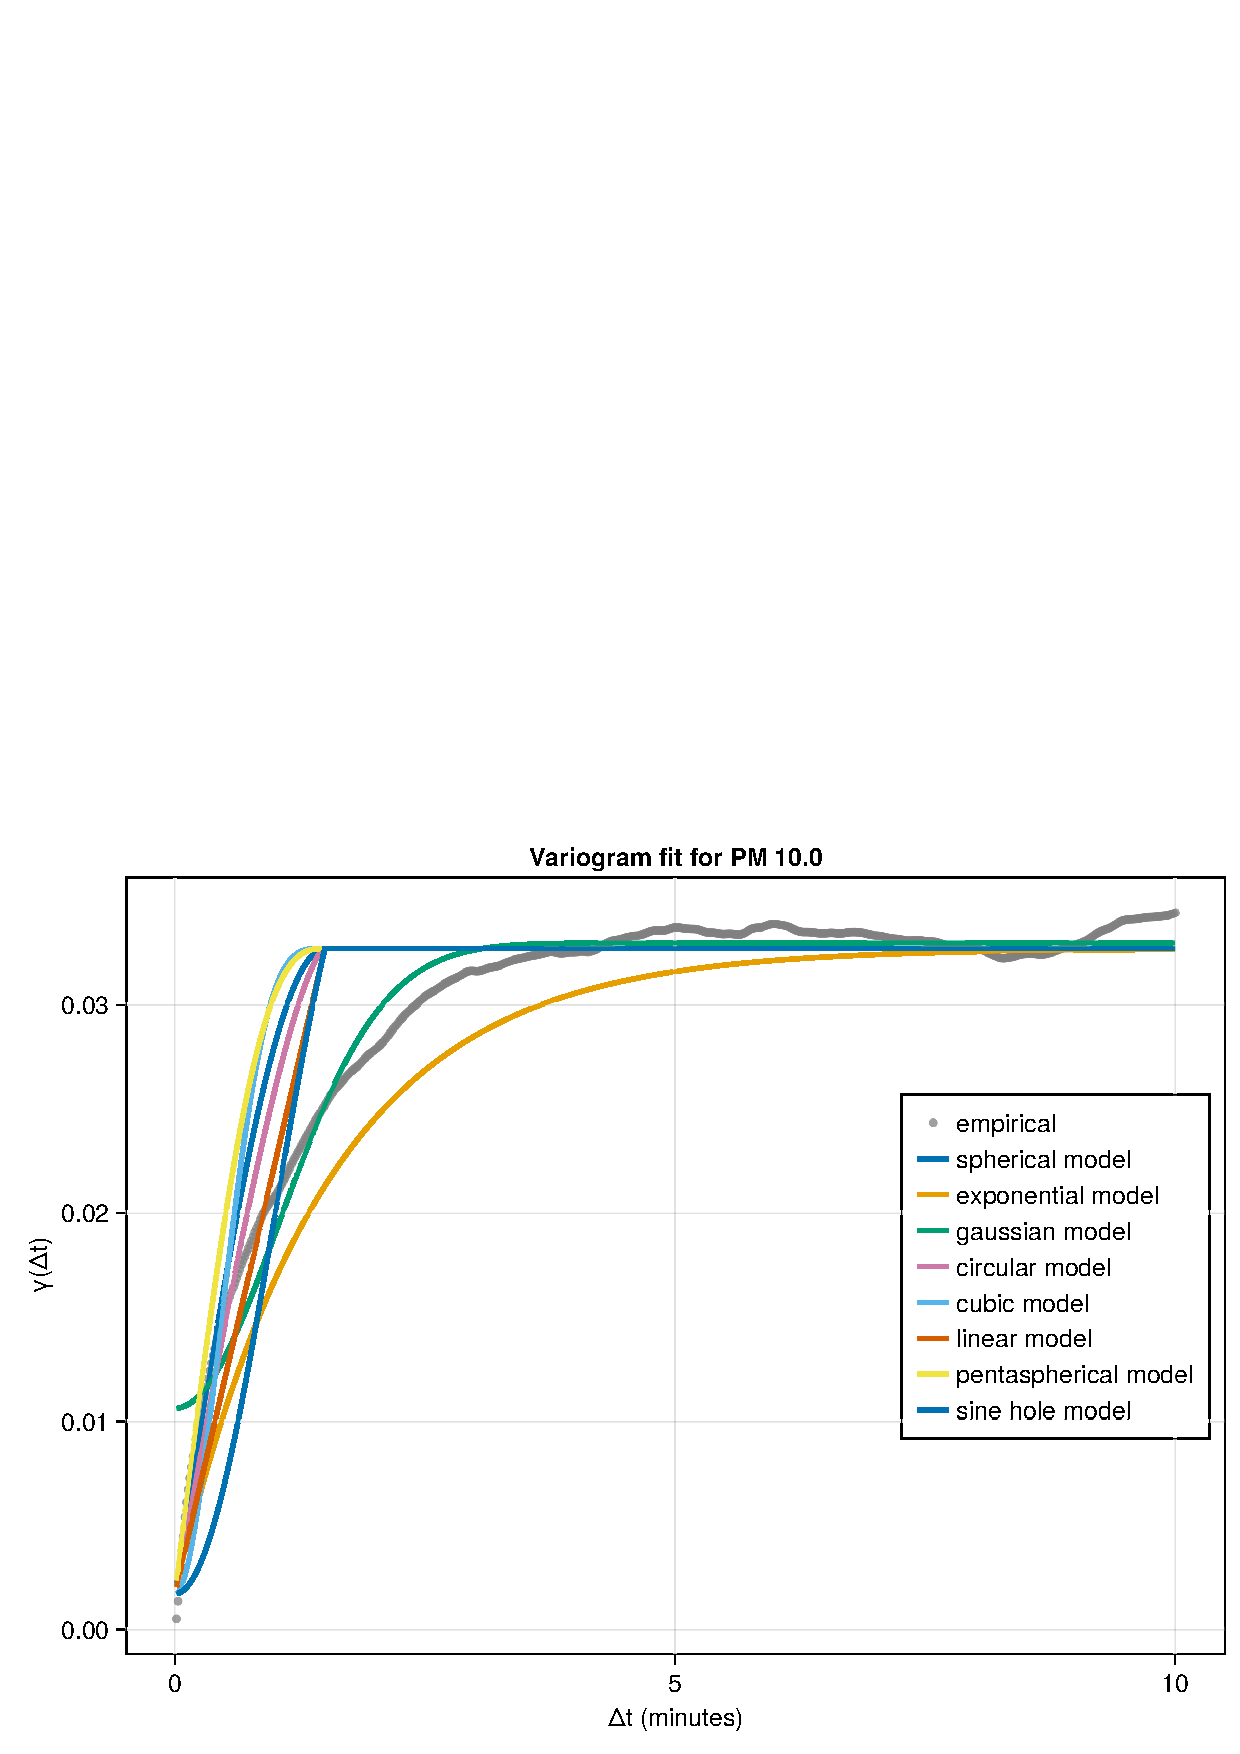
\includegraphics[width=0.85\columnwidth]{time-series/variogram/single-day/γ-PM 10.0_single-day.pdf}
  \caption{The empirical variogram and a variety of model fits obtained for the a PM $10.0$ single-day time series}
  \label{fig:pm10-variogram-fits}
\end{figure}

\subsection{Next Steps}

The next step is to apply the methods to examine the trends in uncertainty estimates for each of the models for a longer period of time (like a year) for a handful of sensors. Do we see any trends that suggest seasonal variability in the uncertainty or a general trend that might suggest end of life for the sensors? 



\section{Physics Informed modeling techniques for Air Quality Data}
%% \subsection{Embedding Theorems}
%% Discuss Taken's embedding theorem and other relevant information for the time-series work.
%% \subsection{Koopman Theory}
%% Give an overview of continuous and discrete Koopman operator theory.
\subsection{A Hybrid HAVOK UDE Approach}

Motivating example: the Lorenz attractor.

\begin{figure}[h]
  \centering
  \includegraphics[width=0.85\columnwidth]{time-series/HAVOK/lorenz/havok/attractors1.png}
  \caption{Comparing the original Lorenz attractor (left) to the embedded attractor learned after performing the SVD (right). Color indicates the time along the trajectory.}
\end{figure}

\begin{figure}[h]
  \centering
  \includegraphics[width=0.85\columnwidth]{time-series/HAVOK/lorenz/havok/eigenmodes.pdf}
  \caption{Eigenmodes of the embedded attractor extracted from the SVD.}
\end{figure}

\begin{figure}[h]
  \centering
  \includegraphics[width=0.85\columnwidth]{time-series/HAVOK/lorenz/havok/heatmap.pdf}
  \caption{Heatmap of the linear Koopman operator together with the forcing activation.}
\end{figure}

\begin{figure}[h]
  \centering
  \includegraphics[width=0.85\columnwidth]{time-series/HAVOK/lorenz/havok/timeseries_reconstructed.pdf}
  \caption{The reconstructed timeseries for $v_1$ via the learned HAVOK model.}
\end{figure}

\begin{figure}[h]
  \centering
  \includegraphics[width=0.85\columnwidth]{time-series/HAVOK/lorenz/havok/scatterplot.pdf}
  \caption{A scatterplot of the resulting HAVOK fit}
\end{figure}

\begin{figure}[h]
  \centering
  \includegraphics[width=0.85\columnwidth]{time-series/HAVOK/lorenz/havok/forcing-stats.pdf}
  \caption{The statistics of the learned forcing function. The sharpness of the distribution (in comparison to a Normal distribution) indicates that the forcing is \textit{intermittent}}
\end{figure}

\begin{figure}[h]
  \centering
  \includegraphics[width=0.85\columnwidth]{time-series/HAVOK/lorenz/havok/v1_forcing_identified.pdf}
  \caption{The time series for $v_1$ marked where the forcing function is above a specified threshold.}
\end{figure}


\begin{figure}[h]
  \centering
  \includegraphics[width=0.85\columnwidth]{time-series/HAVOK/lorenz/havok/attractor_w_forcing.png}
  \caption{The embedded attractor colored by the presence of external forcing.}
\end{figure}

Now what happens if we attempt this procedure on a real, noisy dataset:



\begin{figure}[h]
  \centering
  \includegraphics[width=0.85\columnwidth]{time-series/HAVOK/sharedair/havok/attractor.png}
  \caption{The embedded attractor for PM $2.5$ time-series data.}
\end{figure}


\begin{figure}[h]
  \centering
  \includegraphics[width=0.85\columnwidth]{time-series/HAVOK/sharedair/havok/heatmap.pdf}
  \caption{Heatmap of the linear Koopman operator together with the forcing activation.}
\end{figure}


\begin{figure}[h]
  \centering
  \includegraphics[width=0.85\columnwidth]{time-series/HAVOK/sharedair/havok/timeseries_reconstructed__r-18__c-10.pdf}
  \caption{The reconstructed time-series for the first three embedding coordinates using the HAVOK fit.}
\end{figure}

\begin{figure}[h]
  \centering
  \includegraphics[width=0.85\columnwidth]{time-series/HAVOK/sharedair/havok/timeseries_reconstructed_zoomed-in.pdf}
  \caption{A zoomed in view of the same time-series reconstruction for the first $2.5$ hours showing a very decent fit. Some kind of error appears to be accumulating over time.}
\end{figure}

\begin{figure}[h]
  \centering
  \includegraphics[width=0.85\columnwidth]{time-series/HAVOK/sharedair/havok/v1_forcing_identified.pdf}
  \caption{The first embedding coordinate with forcing above a critical threshold identified.}
\end{figure}

\begin{figure}[h]
  \centering
  \includegraphics[width=0.85\columnwidth]{time-series/HAVOK/sharedair/havok/attractor_w_forcing.png}
  \caption{The original attractor now colored by external forcing above a threshold.}
\end{figure}


Now we can justify the use of a UDE approach to fit missing non-linear terms once we have a trained HAVOK model.



\subsection{Hamiltonian Neural Networks}

An alternative approach to modeling the time series is to consider a system under no external forcing. We can describe the dynamics for this system using \textit{some} set of generalized coordinates via Hamiltons equations. Now we suggest to learn an appropriate set of coordinates $(q,p)$ via an auto-encoder structure so that we can then \textit{learn} a Hamiltonian function for which these coordinates satisfy Hamilton's equations for short times. Once we have this model, we can then analyze the motion of our systems state on the Hamiltonian surface. When there is some kind of external forcing driving us away from the level sets of $H$ can we expect to see large jumps in PM concentration? Further, does the Hamiltonian function learned for a single system generalize well to multiple distributed sensors? 

\begin{figure}[h]
  \centering
  \includegraphics[width=0.85\columnwidth]{time-series/HNN/hamiltonian_cn_1--2022.pdf}
\end{figure}







%% \begin{itemize}
%% \item Uncertainty Estimation Via Time Series Sampling
%% \item Types Of Uncertainty
%% \item Instrument Uncertainty
%% \item Representativeness Uncertainty
%% \item Variograms
%% \item Mutual Information
%% \item Auto-correlation
%% \item Time Series Chaos
%% \item What is Chaos?
%% \item Lyapunov Exponents
%% \item Fractal Dimension
%% \item Koopman Operator Theory
%% \item Time Series Modeling Methods
%% \item Token-Hankel Delay Embeddings
%% \item Embedding Theorems (are magic)
%% \item Determination of Optimal Lag
%% \item Determination of Intrinsic Dimension (kind of unnecessary given *large enough* embedding)
%% \item DMD and HAVOK
%% \item Hamiltonian Neural Networks
%% \item Time Series Classification
%% \item Considerations for Batching of Time Series for ML Models
%% \item K-means Clustering
%% \item Self Organizing Maps
%% \item Generative Topographic Maps
%% \item Chaos Classification via HAVOK
%% \item Symplectic and Normal Gradients for HNN
%% \item Motivating Example: Lorenz63 System
%% \item Origin of Lorenz System
%% \item Time Scale Analysis and Variography
%% \item Embedding
%% \item Modeling
%% \item Classification
%% \item Real Example 1: PM Data
%% \item Origin of Lorenz System
%% \item Time Scale Analysis and Variography
%% \item Embedding
%% \item Modeling
%% \item Classification
%% \item Real Example 2: Biometric Data
%% \item Origin of Lorenz System
%% \item Time Scale Analysis and Variography
%% \item Embedding
%% \item Modeling
%% \item Classification
%% \item Real Example 3: Stock Market Analysis
%% \item Origin of Lorenz System
%% \item Time Scale Analysis and Variography
%% \item Embedding
%% \item Modeling
%% \item Classification
%% \end{itemize}
